\providecommand{\topdir}{..}
\documentclass[../main.tex]{subfiles}

\ifSubfilesClassLoaded{
  \externaldocument[main-]{../main}
  \externaldocument[fm-]{../00_front_matter/front_matter}
  \externaldocument[intro-]{../01_introduction/introduction}
  \externaldocument[l96-]{../02_lorenz96/lorenz96}
  \externaldocument[rb-]{../03_rayleigh_benard/rayleigh_benard}
  \externaldocument[eval-]{../05_evaluation/evaluation}
  \externaldocument[conc-]{../06_conclusion/conclusion}
  \externaldocument[app-]{../07_appendix/appendix}

  \setcounterref{chapter}{main-chap:tendencies}
  \addtocounter{chapter}{-1}
}{}

\begin{document}

\ifSubfilesClassLoaded{
    \frontmatter
    \tableofcontents
    \mainmatter
}{}

\chapter{Analysis and modelling of subgrid tendencies}
\label{chap:tendencies}
\setlength{\epigraphwidth}{.45\textwidth}
\epigraphhead[0.1\textheight]{
    \epigraph{%
        Good approximations often lead to better ones.
    }{\emph{Mathematical Methods in Science}\\George P\`{o}lya, 1977}
}

\todo{introductory paragraph: why am I doing this?}
\todo{mention Alieva paper more}

In \cref{rb-chap:rayleigh_benard} I investigated the resolution dependence
of several metrics in order to choose the resolutions of the fine ``truth''
model and the coarse ``control'' model needed for data-driven parametrisation.
\cref{tab:final_resolutions} shows the final choices; for the remainder
of this thesis, the terms ``fine model'' and ``coarse model'' will refer
to the settings shown in the Table.

\begin{table}[ht]
\centering
\begin{tabular}{l l l}
    \toprule
    & \textbf{Fine model} & \textbf{Coarse model} \\
    \midrule
    $N_x$ & 2048 & 256 \\
    $N_z$ & 256 & 64 \\
    $\Delta t$ & $\SI{1.0e-3}{}$ & $\SI{5.333e-3}{}$ \\
    \bottomrule
\end{tabular}
\caption{
    Resolutions $(N_x, N_z)$ and time steps $\Delta t$ chosen for the fine and
    coarse models.
}
\label{tab:final_resolutions}
\end{table}


\section{Calculation of subgrid tendencies} \label{sec:calculation}
The workflow used to calculate the subgrid tendencies is described below and
illustrated as a flowchart in \cref{fig:method}, which uses the same numbering
to show the order of the steps. \todo{refer to literature}
\begin{enumerate}
    \item\label[step]{itm:fine_model} The fine model was integrated for 300
        time units, the initial condition being the end of the $2048 \times
        256$ simulation in \cref{rb-chap:rayleigh_benard}. Every 3 time units,
        the model state was saved, and then saved again one time step later.
        This resulted in a dataset of 100 pairs of snapshots separated by 3
        time units. An interval of 3 time units was chosen as it was the
        approximate decorrelation time of the model variables (see
        \cref{app-sec:snapshot_freq}); using a shorter interval would result in
        saving redundant information.
    \item\label[step]{itm:coarse_grain} Each pair of snapshots was
        \emph{coarse-grained}, reducing its spatial resolution to that of the
        coarse model. The nature of the coarse-graining operation warrants
        special attention and is discussed separately in
        \cref{sec:coarse_graining}.
    \item\label[step]{itm:coarse_model} The first coarse-grained snapshot in
        each pair was input as an initial condition for the coarse model. The
        coarse model integrated for one time step only, and the resulting
        state---the coarse model's prediction for the large-scale state after
        one time step---was saved.
    \item\label[step]{itm:true_tend} The first coarse-grained snapshot in each
        pair from \cref{itm:coarse_grain} was subtracted from the second
        and the difference divided by the fine model's time step, giving the
        \emph{true coarse tendency} (i.e., the true time derivative of the
        large-scale state as calculated by the fine model).
    \item\label[step]{itm:pred_tend} The first coarse-grained snapshot in each
        pair from \cref{itm:coarse_grain} was subtracted from the coarse model
        prediction produced in \cref{itm:coarse_model} and the difference
        divided by the coarse model's time step, giving the tendency predicted
        by the coarse model (i.e., its prediction of the time derivative of the
        large-scale state).
    \item\label[step]{itm:subgrid_tend} Finally, the coarse model predicted
        tendencies from \cref{itm:pred_tend} were subtracted from the true
        coarse tendencies from \cref{itm:true_tend}, producing the
        \emph{subgrid tendencies}. These measure the error (or, more precisely,
        minus the error) in the coarse model's prediction of the time
        derivative of the large-scale state, and would be identically zero for
        a perfect coarse model.
\end{enumerate}

The goal will be to approximate the subgrid tendencies (labelled
``predictand'' in \cref{fig:method}) as functions of the coarse state (labelled
``predictor''). In \cref{eval-chap:evaluation}, I construct a new coarse model
that adds the approximate subgrid tendencies to the original predicted
tendencies, thereby obtaining a better approximation to the true coarse
tendency. When integrated, the new coarse model should, in principle,
yield a solution that more closely matches the coarse-grained solution of
the fine model.

\begin{figure}[ht]
    \centering
    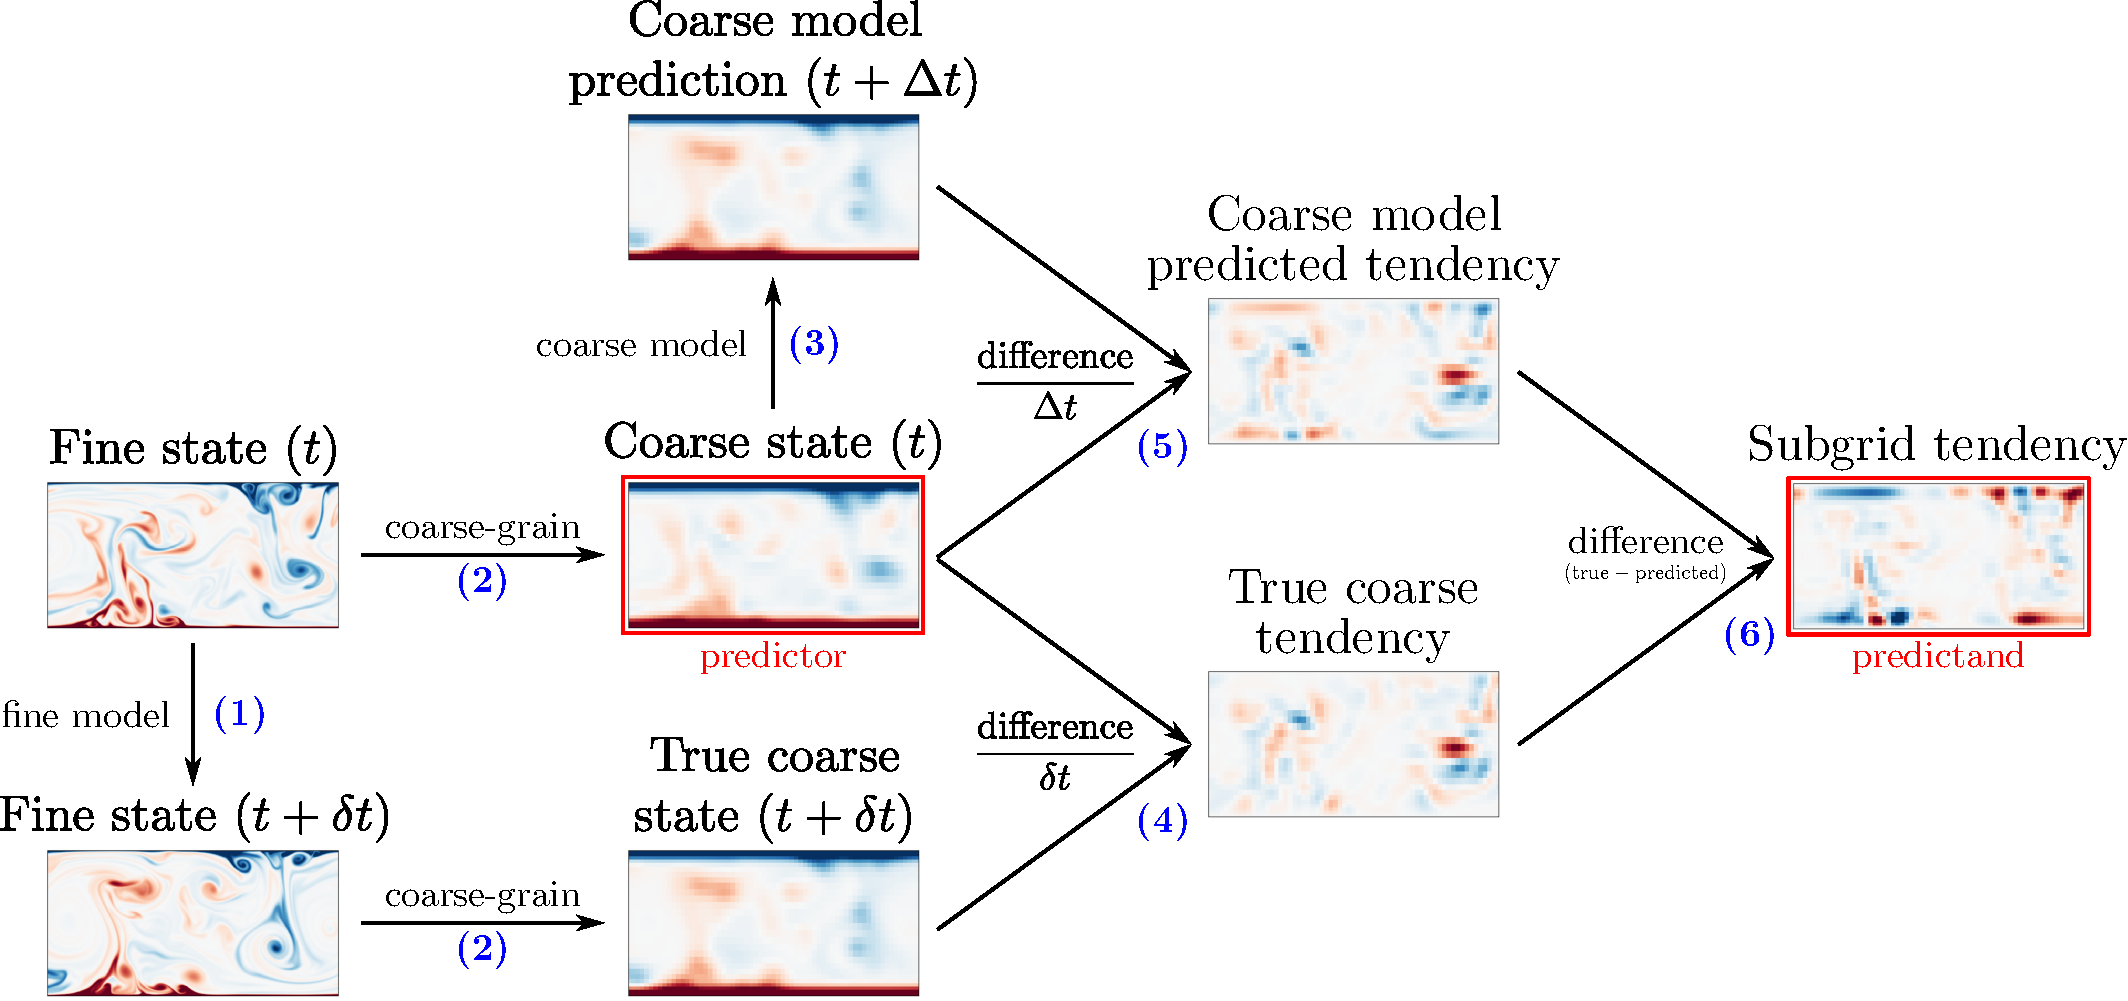
\includegraphics[width=\linewidth]{figures/method_v2.pdf}
    \caption{
        Flowchart illustrating the procedure used to calculate subgrid
        tendencies. The plots show an example of the workflow being applied to
        the temperature data but are for illustrative purposes only. The blue
        numbers correspond to the steps described in the text.
    }
    \label{fig:method}
\end{figure}


\section{Choice of coarse-graining method} \label{sec:coarse_graining}
Coarse-graining is the process of reducing a gridded dataset onto a
lower-resolution grid, and it is required at \cref{itm:coarse_grain} of the
workflow described in \cref{sec:calculation}. It was found that the choice of
coarse-graining method was a major influence on the quality of the calculated
subgrid tendencies; this is the consequence of a subtle issue that may seem
purely semantic at first but in fact has important practical implications.

In general, the output of a coarse (i.e., reduced-order) model is meant to
approximate a certain \emph{representation} of the output of a chosen fine
model. To give three concrete examples, the coarse model might seek to
reproduce (a) the values of the high-resolution fields on a sparser grid of
points, or (b) the averages over a set of larger grid boxes, or (c) the first
$N$ coefficients of the discrete Fourier transform (where $N$ is less than the
number of coefficients needed to fully determine the original fields). The
modeller has the freedom choose a representation, which in turn determines how
the output of the coarse model should be interpreted. The choice of
representation also implicitly determines a coarse-graining operation: a map
from the state space of the fine model to the state space of the coarse model
that isolates the necessary large-scale information and discards the rest.
Referring to the previous examples, option (a) calls for an operation that
simply discards, say, three out of every four or nine out of ten grid points.
Option (b) calls for the grouping and averaging of the grid points that lie
within each large grid box. Option (c) calls for the truncation of fine fields
at the $N$th coefficient in Fourier space.

The key lesson that was learnt during the course of this work is that the
chosen representation and coarse-graining method must be appropriate to the
nature of the coarse model. In this work, the coarse model was a Dedalus solver
that, in \cref{itm:coarse_model} of the workflow in \cref{sec:calculation},
received gridded initial condition data in real space and integrated the
governing equations forward in time using the same numerical method as the
fine model. This gave rise to two constraints on the coarse-graining method:
\begin{enumerate}
    \item The coarse-grained initial condition must be well-resolved on the
        coarse model's grid. Numerical solution algorithms for PDEs assume
        (e.g., by approximating derivatives as finite differences) that the
        solution is well-resolved on the discrete model grid, and can become
        unstable or produce output marred by artefacts if this condition is not
        met.
    \item The initial condition must respect physical constraints, namely the
        divergence-free condition \cref{rb-eqn:incompressible} and the boundary
        conditions \crefrange{rb-eqn:bc_bot}{rb-eqn:bc_sides}. A numerical
        algorithm cannot be expected to behave predictably when presented with
        unphysical initial conditions.
\end{enumerate}

During the development of this study, before the above requirements were known,
coarse-graining was performed by averaging the fine grid points that lay within
each coarse grid box (a method known within the Earth sciences as
\emph{first-order conservative remapping} or \emph{regridding} because it
preserves mean values; see \cite{jones1999}).
\cref{fig:coarse_graining_example}, illustrating the application of first-order
conservative regridding to sample temperature data, demonstrates that the
result is not very well-resolved on the coarse grid; in many places, adjacent
grid points have sharp differences in temperature. First-order conservative
regridding is also not guaranteed to preserve boundary values or the
divergence-free nature of the velocity field. Consequently, the tendencies
obtained from the coarse model in \cref{itm:pred_tend} of the workflow suffered
from noise and numerical artefacts that propagated to the subgrid tendencies in
\cref{itm:subgrid_tend}. With the signal of interest obscured, it was
impossible to model the subgrid tendencies as functions of the coarse state.

It was evident that the coarse-graining method needed to involve a smoothing
operation of some kind. However, most conventional smoothing methods, such as
Gaussian filtering, also fail to preserve the boundary and divergence-free
conditions. The solution to this problem was to supply each snapshot of the
fine model state as an initial condition to an appropriate system of PDEs,
chosen so that the integration of the system would have a smoothing effect on
the initial condition data. The key advantage of this approach is that the
boundary and divergence-free conditions can be explicitly enforced.

The choice of PDEs to achieve this was inspired by classical Gaussian
filtering. Recall that a Gaussian filter convolves input data with a filter
kernel that takes the form of a Gaussian function, which also happens to be the
Green's function for the heat equation $\partial \psi / \partial t = \nabla^2
\psi$ in an \emph{infinite} domain. It follows that heat equations of some form
on the \emph{finite} domain of the \rb{} problem (whose Greeen's functions are
not Gaussian) will have a similar smoothing effect while preserving the
required boundary conditions. The appropriate equation for smoothing the
temperature field $\theta$ is therefore
\begin{equation}
    \label{eqn:diffusion_theta}
    \pdiff{\theta}{t} = \nabla^2 \theta
\end{equation}
on $[0, \Gamma] \times [0, 1]$ with $\theta(z=0) = +1/2$, $\theta(z=1) = -1/2$
and $\theta(x=0) = \theta(x=\Gamma)$. It is tempting to propose an equation of
the same form, $\partial \vec{u} / \partial t = \nabla^2 \vec{u}$, for the
velocity field, but its solution on the finite domain would not necessarily
preserve $\grad \cdot \vec{u} = 0$. By analogy to the incompressible
Navier-Stokes equations, it is necessary to introduce a ``pressure'' term
$-\grad\pi$ on the right-hand side, with the additional field $\pi(x,z)$ giving
an additional degree of freedom that allows one to impose $\grad \cdot \vec{u}
= 0$ without over-determining the problem. The velocity field is thus
smoothed by the equations
\begin{align}
    \label{eqn:diffusion_u}
    \pdiff{\vec{u}}{t} &= -\grad\pi + \nabla^2 \vec{u} \quad \text{and} \\
    \label{eqn:diffusion_continuity}
    \grad \cdot \vec{u} &= 0
\end{align}
on $[0, \Gamma] \times [0, 1]$ with $\vec{u}(z=0) = \vec{u}(z=1) = \vec{0}$ and
$\vec{u}(x=0) = \vec{u}(x=\Gamma)$. The equations
\crefrange{eqn:diffusion_theta}{eqn:diffusion_continuity} were integrated
numerically on the same grid as the fine model using a solver that was
straightforwardly implemented in Dedalus.

Once the high-resolution data had been smoothed using the method described
above, all that remained was to downsample the result to the resolution of the
coarse model. Downsampling was handled by Dedalus via truncation in spectral
coefficient space. To summarise, the coarse-graining workflow is as follows:
\begin{enumerate}
    \item\label[step]{itm:coarse_grain_input} Input a high-resolution snapshot
        as the initial condition for the solver of
        \crefrange{eqn:diffusion_theta}{eqn:diffusion_continuity}.
    \item Integrate the solver for $\SI{e-3}{}$ time units (the duration that
        was found to produce the necessary amount of smoothing) in steps of
        $\SI{2e-4}{}$ time units.
    \item Downsample the final state to the resolution of the coarse model
        and save the result.
    \item Reset the solver and return to \cref{itm:coarse_grain_input} to
        coarse-grain the next high-resolution snapshot.
\end{enumerate}

\cref{fig:coarse_graining_example} compares the results of the improved
coarse-graining method and first-order conservative regridding for the
temperature field. Close inspection of the figure shows that the improved
coarse-graining method produces smooth results that are well-resolved on the
coarse grid, in contrast to first-order conservative regridding.

\begin{figure}[ht]
    \centering
    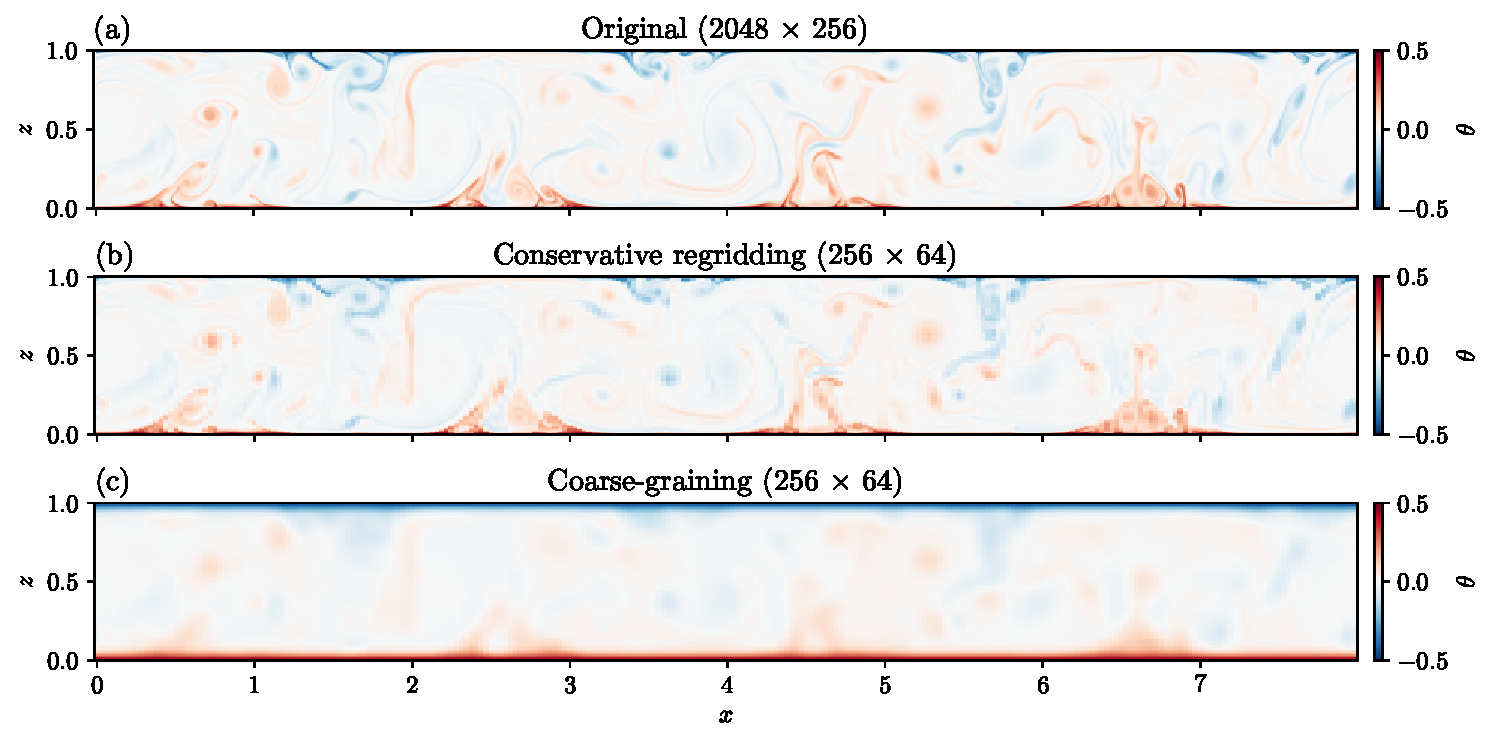
\includegraphics[width=\linewidth]{figures/coarse_graining_example.pdf}
    \caption{
        \textbf{(a)} A snapshot of the temperature field in a simulation with
        $2048 \times 256$ resolution; \textbf{(b)} the field in (a) after
        first-order conservative regridding to $256 \times 64$ (poorly
        resolved on the coarse grid); \textbf{(c)} the field in (a) after
        coarse-graining to $256 \times 64$ using the method in the text
        (smooth and well-resolved on the coarse grid).
    }
    \label{fig:coarse_graining_example}
\end{figure}


\section{Analysis of subgrid tendencies} \label{sec:subgrid_analysis}
In this section, I will analyse the subgrid tendency data by plotting joint
histograms of subgrid tendencies (the predictands) against coarse state
variables and other quantities derived from the coarse state variables (the
predictors). At each time step, predictor and predictand fields were sampled
using linear interpolation at $256 \times 64 = 16384$ random, uniformly
distributed points in the domain\footnote{It is necessary to randomly sample
the fields in this way, rather than using the raw gridded data, to remove
artefacts that appear in the histograms when large groups of sampling points
share the exact same vertical position $z$.}.

The obvious first step is to plot joint histograms for the subgrid tendencies
of $u$, $w$ and $\theta$ against the values of $u$, $w$ and $\theta$
themselves. \cref{fig:subgrid_vs_vars} shows all $3 \times 3 = 9$ possible
histograms, as well as the marginal distributions. There are no immediately
obvious correlations; each joint distribution appears similar to the product of
its corresponding marginal distributions. This finding contrasts with the
well-known results for the Lorenz '96 model that were discussed in
\cref{l96-chap:lorenz96}. While \cref{l96-fig:wilks2005_regression} showed that
the subgrid tendencies of Lorenz '96 can, to a large extent, be be predicted
directly from the values of the resolved variables, the problem is evidently
more complex for \rb{} convection.

\begin{figure}[ht]
    \centering
    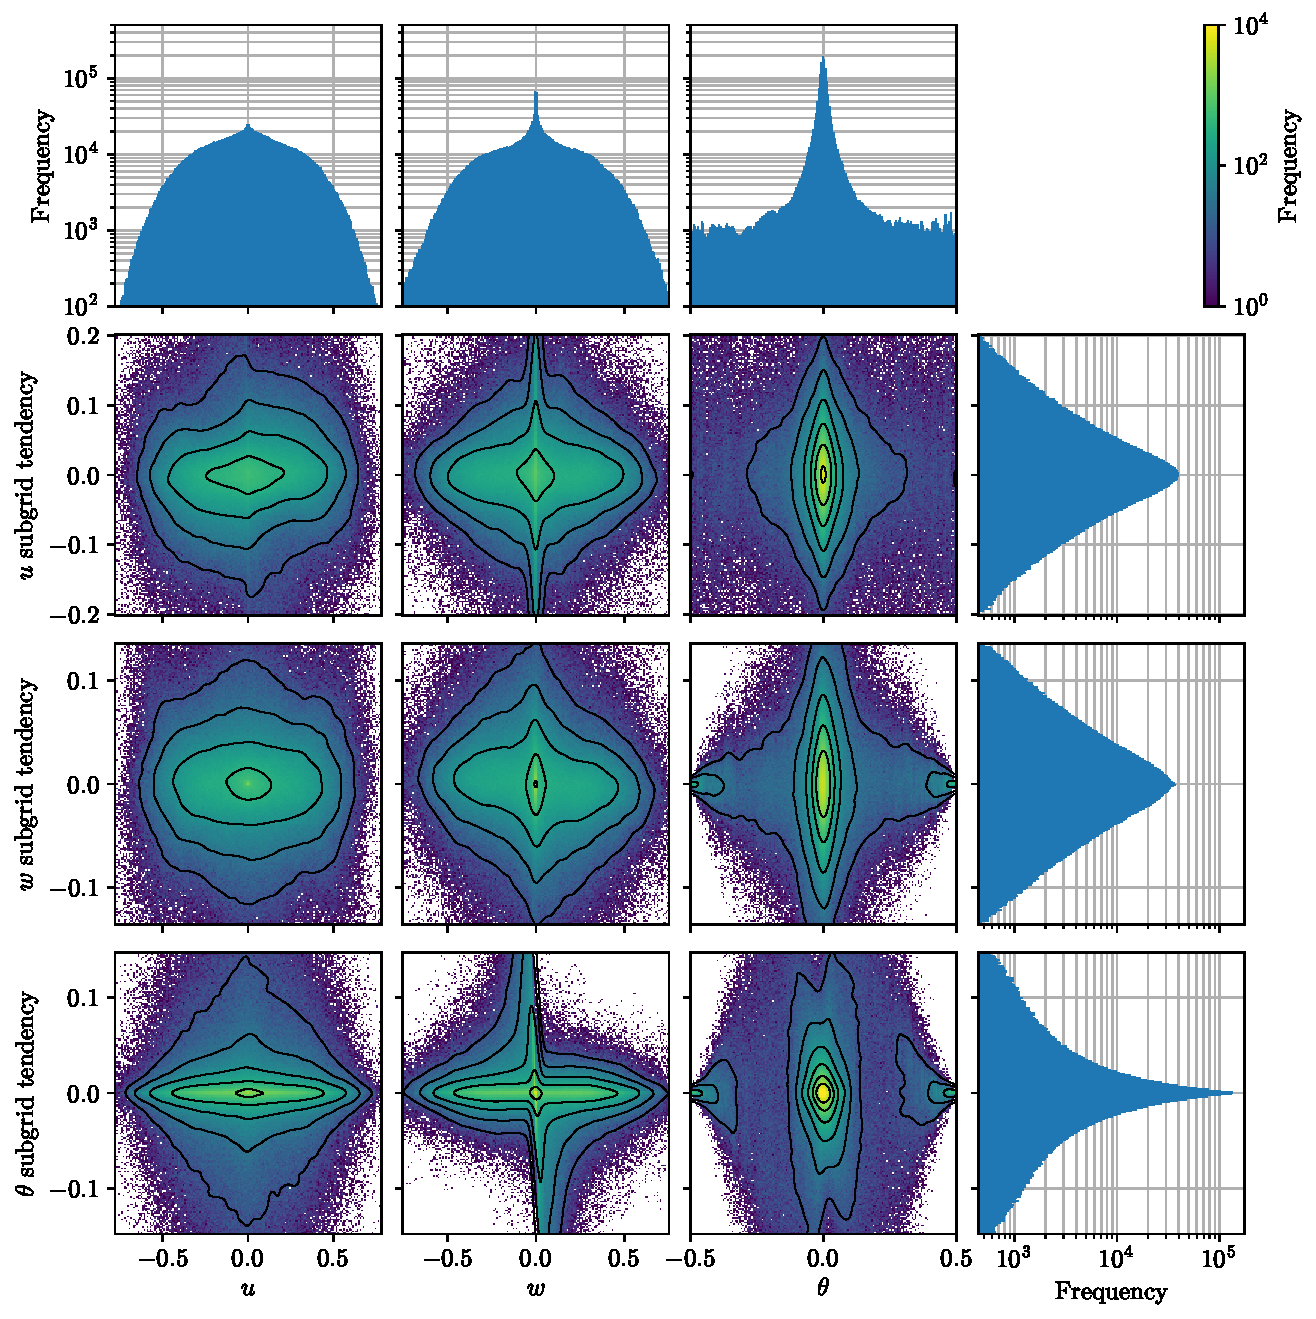
\includegraphics[width=\linewidth]{figures/subgrid_vs_vars.pdf}
    \caption{
        Joint histograms of the $u$, $w$ and $\theta$ subgrid tendencies
        against the values of $u$, $w$ and $\theta$ themselves (main 3-by-3
        grid of pseudocolour plots); and marginal distributions (top row and
        right column). Note that the joint histograms use a logarithmic
        colour scale; smoothed contours (black) are plotted at constant
        intervals in log-space.
    }
    \label{fig:subgrid_vs_vars}
\end{figure}

Take note, however, of the unusual shape of the joint distribution of the
$\theta$ subgrid tendency against $w$ (bottom row, second from left in
\cref{fig:subgrid_vs_vars}). It does not appear to be a simple product of the
marginal distributions, instead having a slanted linear feature near $w=0$. The
origin of this feature is revealed by conditioning on the vertical coordinate
$z$ (or, in other words, using $z$ as a second predictor in addition to $w$). I
achieve this by plotting, in \cref{fig:theta_vs_w}, a series of joint
histograms, each one using samples from a different horizontal slice of the
domain. When sampling is restricted to $z \in [0.0, 0.1]$ or $z \in [0.9,
1.0]$, a negative correlation is revealed. This means that the coarse model
tends to overestimate the rate of temperature change when the vertical velocity
is positive (requiring a negative subgrid tendency correction) and
underestimate it when the vertical velocity is negative (requiring a positive
correction). This correlation is not present in the middle of the domain,
indicating that the slanted feature in the original hisogram originates in the
boundary layers.

\begin{figure}[ht]
    \centering
    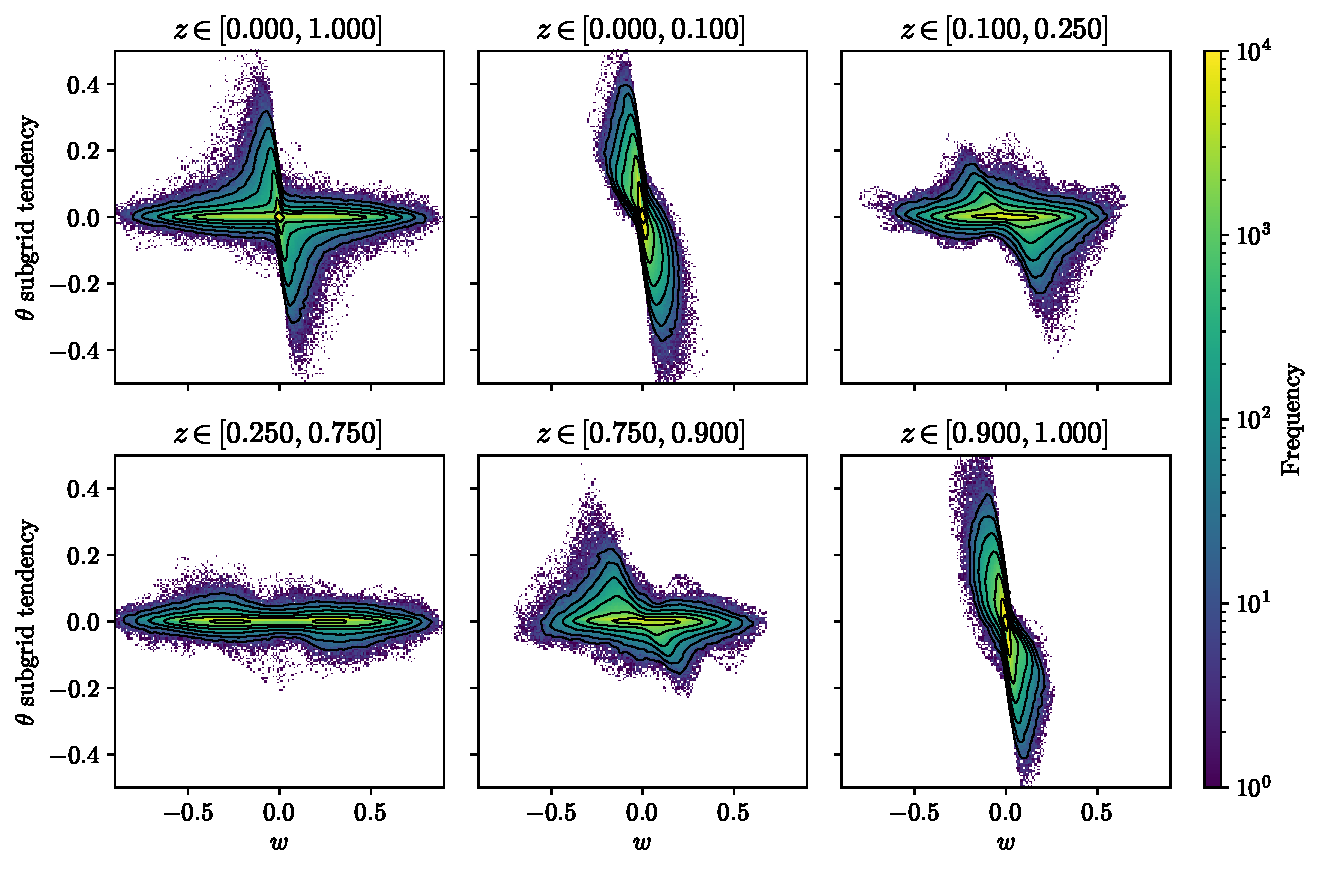
\includegraphics[width=0.9\linewidth]{figures/theta_vs_w.pdf}
    \caption{
        Joint histograms of the $\theta$ subgrid tendency against $w$,
        conditioned on $z$. The top left panel shows the unconditioned
        histogram from \cref{fig:subgrid_vs_vars}; the others only use samples
        from certain horizontal slices of the domain, as indicated by their
        titles.
    }
    \label{fig:theta_vs_w}
\end{figure}

Another option is to use the derivatives of $u$, $w$ and $\theta$ (computed
using finite differences) as predictors.
\crefrange{fig:theta_vs_dudx}{fig:w_vs_dudx} show similar conditional joint
histograms for three of the possible pairings, namely $\theta$ subgrid tendency
against $\partial u/\partial x$, $u$ subgrid tendency against $\partial
u/\partial z$ and $w$ subgrid tendency against $\partial u/\partial x$. These
also reveal correlations that only exist near the top and bottom of the domain;
interestingly, there is a markedly nonlinear correlation for the last pair.
Overall, it is unsurprising that the subgrid tendency statistics are
position-dependent, since the system lacks a vertical translation symmetry.
This is another point of contrast with the Lorenz '96 system (see
\cref{l96-chap:lorenz96}).

Another observation from \cref{fig:theta_vs_w,fig:theta_vs_dudx,fig:u_vs_dudz}
is that the subgrid tendencies of $u$ and $\theta$ both have noticeably larger
variances near the top and bottom of the domain than in the middle. In other
words, the coarse model tends to suffer from larger errors in the near-wall
regions, suggesting that parametrisation may play a more important role in
these places. This supports the findings of \textcite{stevens2010}, who (as
discussed in \cref{rb-sec:metrics}) reported insufficient thermal dissipation
near the side walls in under-resolved simulations of \rb{} convection in a
cylindrical cavity. My result is also reminiscent of recent work by
\textcite{alieva2023}, who, in developing machine-learning-augmented \rb{}
simulations, found that best greater accuracy was achieved when the ML
correction was only applied in the near-wall regions.

\begin{figure}[ht]
    \centering
    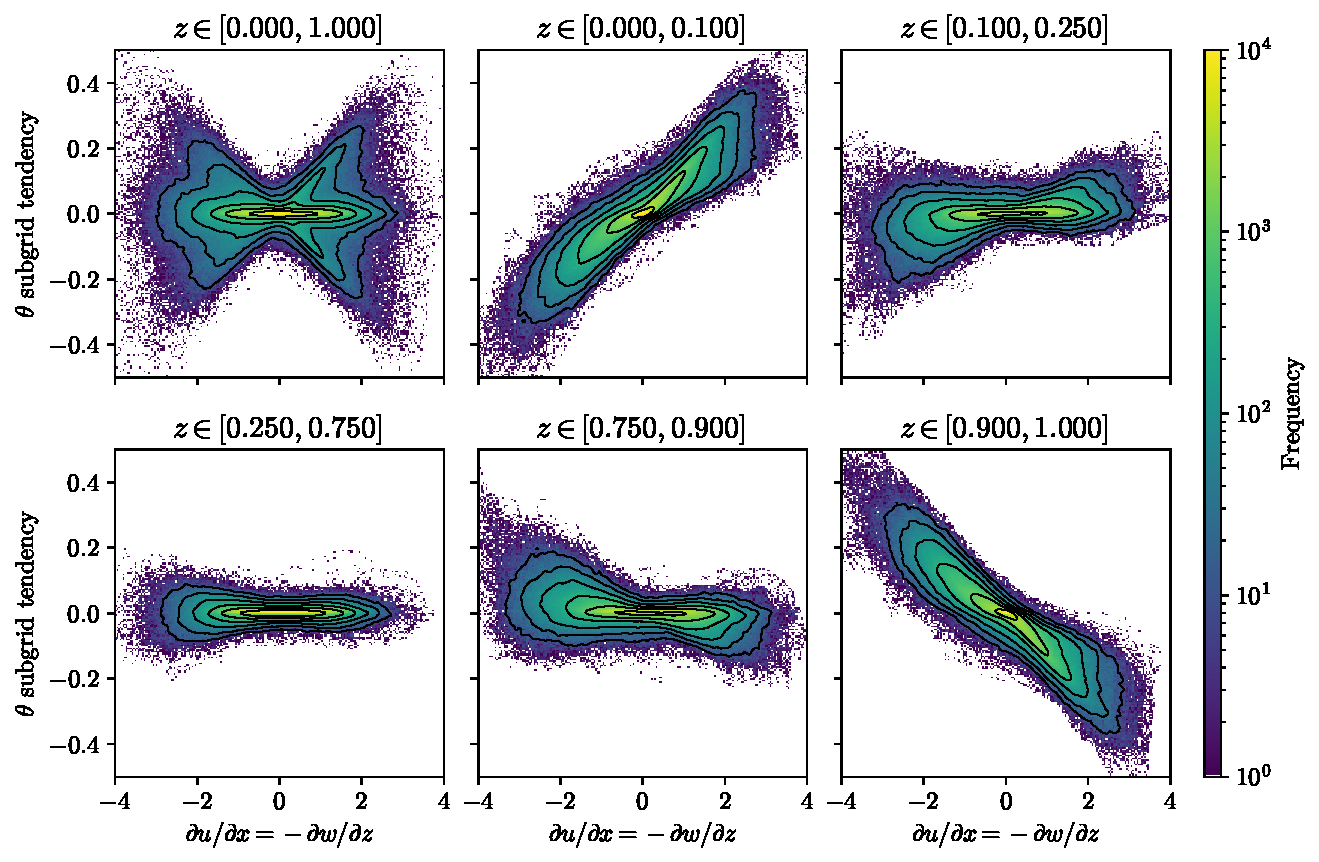
\includegraphics[width=0.9\linewidth]{figures/theta_vs_dudx.pdf}
    \caption{
        The equivalent of \cref{fig:theta_vs_w} for the $\theta$ subgrid
        tendency against $\partial u/\partial x$ (which is equal to
        $-\partial w/\partial z$ due to incompressibility).
    }
    \label{fig:theta_vs_dudx}
\end{figure}

\begin{figure}[ht]
    \centering
    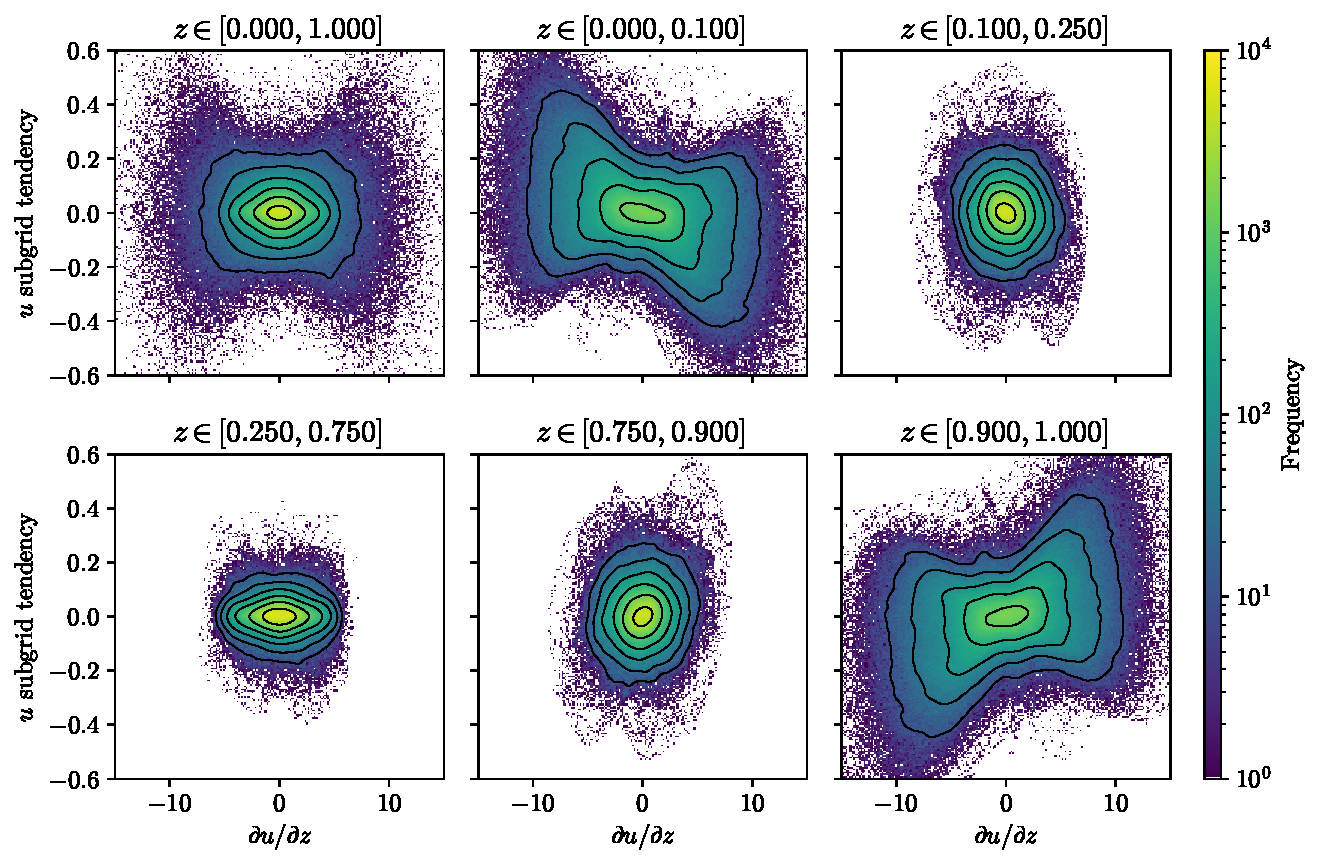
\includegraphics[width=0.9\linewidth]{figures/u_vs_dudz.pdf}
    \caption{
        The equivalent of \cref{fig:theta_vs_w} for the $u$ subgrid
        tendency against $\partial u/\partial z$.
    }
    \label{fig:u_vs_dudz}
\end{figure}

\begin{figure}[ht]
    \centering
    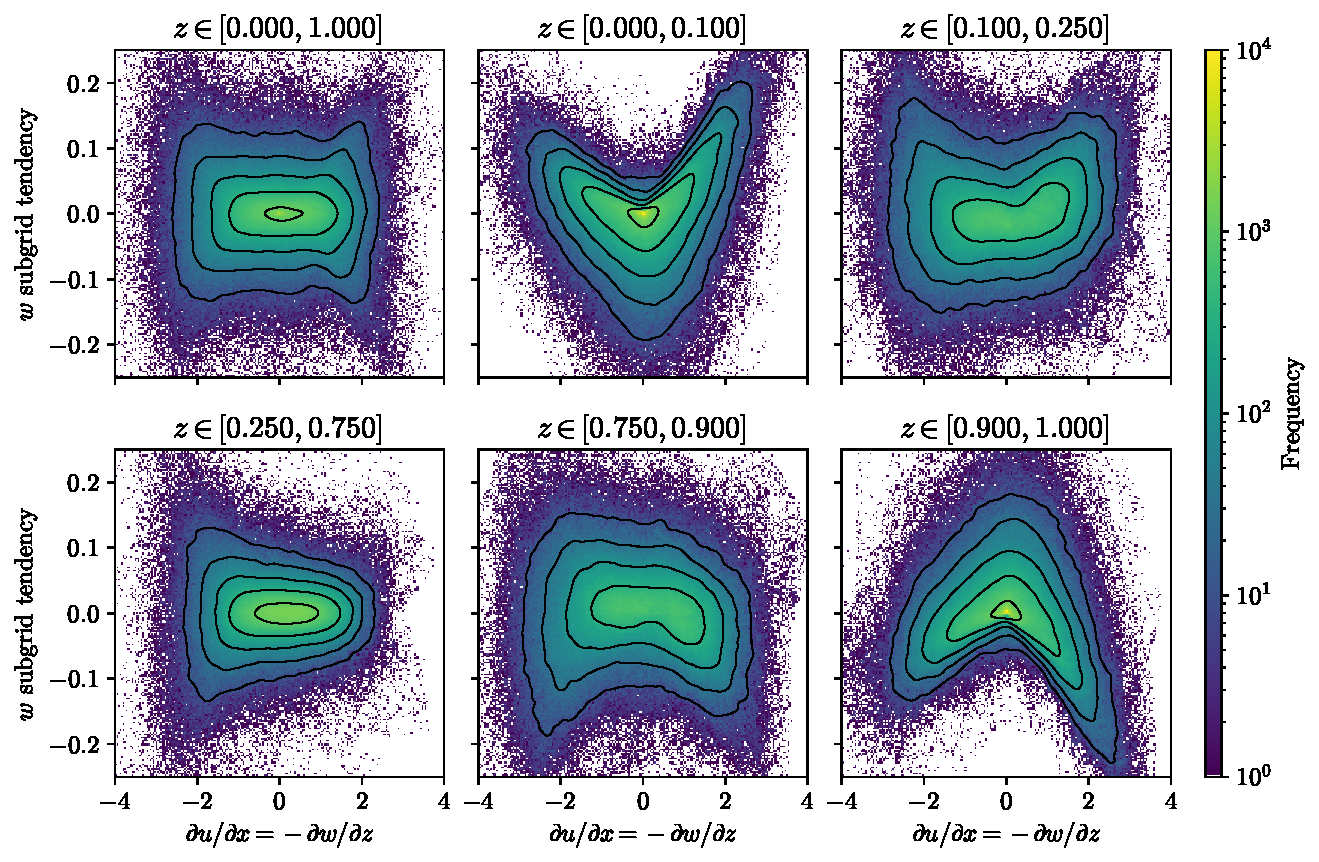
\includegraphics[width=0.9\linewidth]{figures/w_vs_dudx.pdf}
    \caption{
        The equivalent of \cref{fig:theta_vs_w} for the $w$ subgrid
        tendency against $\partial u/\partial x$ (which is equal to
        $-\partial w/\partial z$ due to incompressibility).
    }
    \label{fig:w_vs_dudx}
\end{figure}

\clearpage
Yet another possibility is to use the coarse model's predicted
\emph{tendencies} (calculated in \cref{itm:pred_tend} of
\cref{sec:calculation}) as predictors for the subgrid tendencies. After all,
the tendencies are functions---given by the governing equations
\crefrange{rb-eqn:hyper_momentum}{rb-eqn:hyper_incompressible}---of $u$, $w$,
$\theta$ and their derivatives. I again generate joint histograms, conditioned
on $z$, for each variable's subgrid tendency against its predicted tendency;
these are shown in
\crefrange{fig:theta_subgrid_vs_pred_tend}{fig:w_subgrid_vs_pred_tend}. For all
three variables, a negative linear correlation appears in the near-wall
regions; furthermore, the distributions in these regions appear to lie roughly
along a line with slope $-1$. This is an interesting and unexpected result
because it indicates that the magnitudes of the coarse model's predicted
tendencies systematically exceed the magnitudes of the true tendencies, calling
for subgrid corrections that almost completely cancel the predictions.
Interestingly, there appears to be a slight \emph{positive} correlation in the
middle of the domain for $u$ (\cref{fig:u_subgrid_vs_pred_tend}d) and $w$
(\cref{fig:w_subgrid_vs_pred_tend}d), indicating that the coarse model is
underestimating the magnitudes of the tendencies in this region.

\begin{figure}[ht]
    \centering
    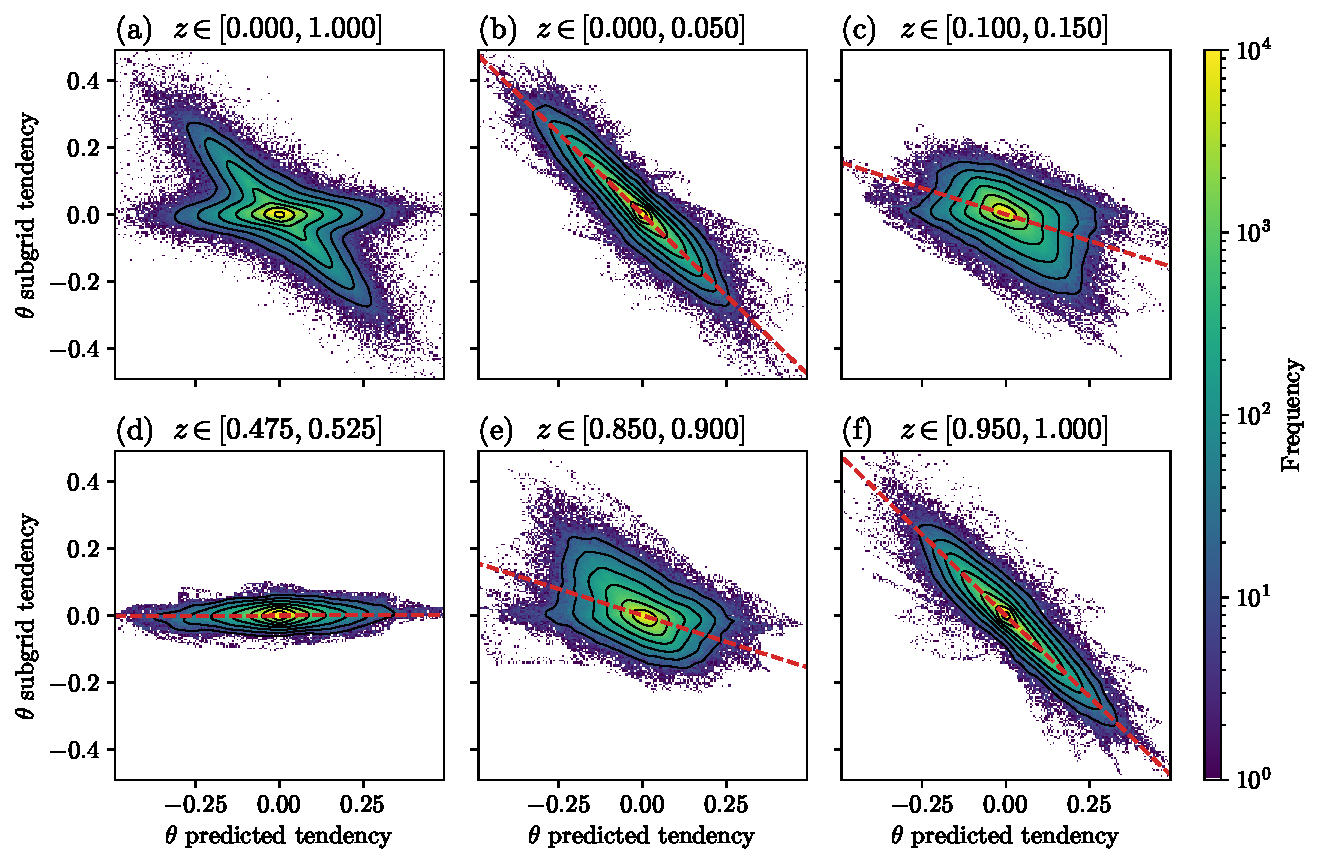
\includegraphics[width=0.95\linewidth]{figures/theta_subgrid_vs_pred_tend.pdf}
    \caption{
        The equivalent of \cref{fig:theta_vs_w} for the $\theta$ subgrid
        tendency against the $\theta$ tendency predicted by the coarse model.
    }
    \label{fig:theta_subgrid_vs_pred_tend}
\end{figure}

\begin{figure}[ht]
    \centering
    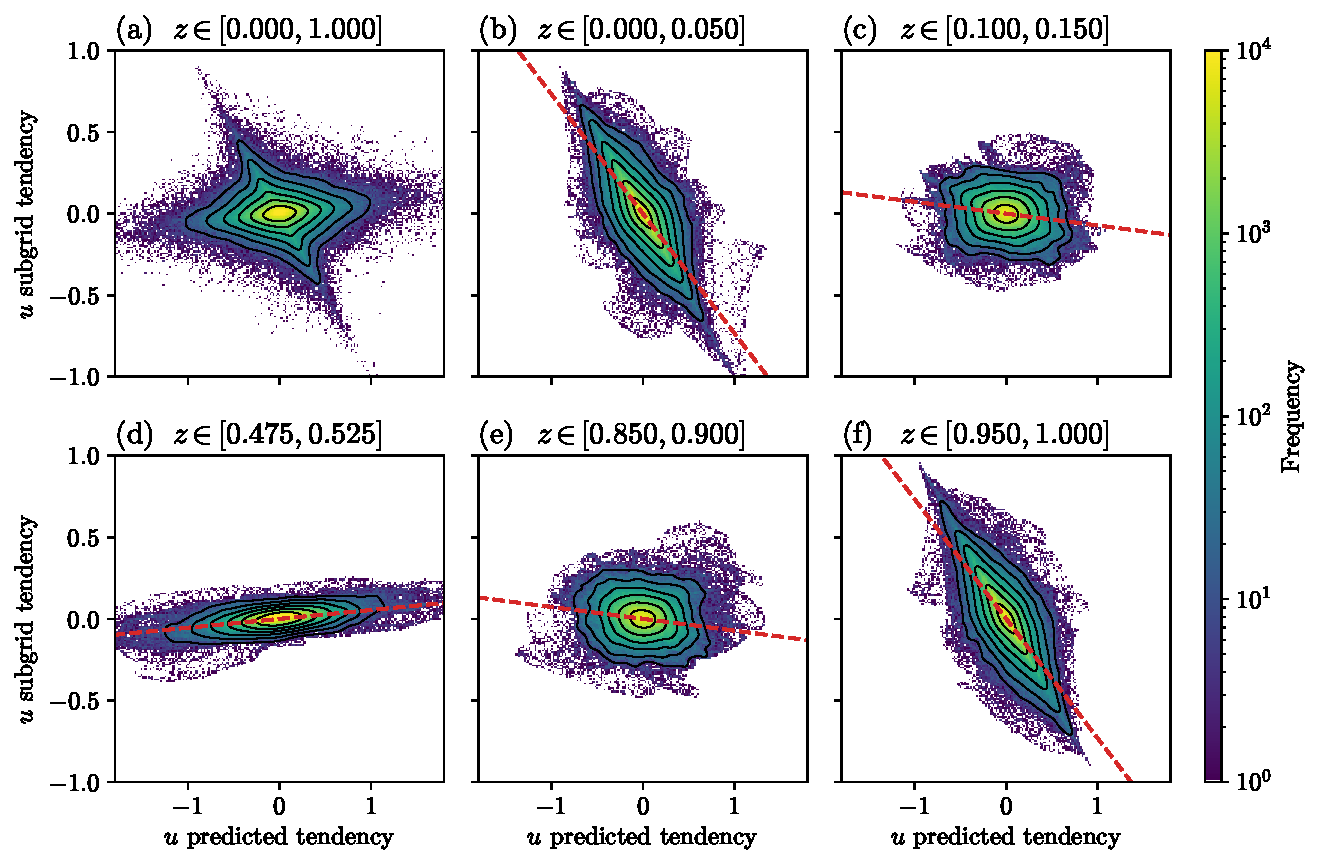
\includegraphics[width=0.95\linewidth]{figures/u_subgrid_vs_pred_tend.pdf}
    \caption{
        The equivalent of \cref{fig:theta_vs_w} for the $u$ subgrid
        tendency against the $u$ tendency predicted by the coarse model.
    }
    \label{fig:u_subgrid_vs_pred_tend}
\end{figure}

\begin{figure}[ht]
    \centering
    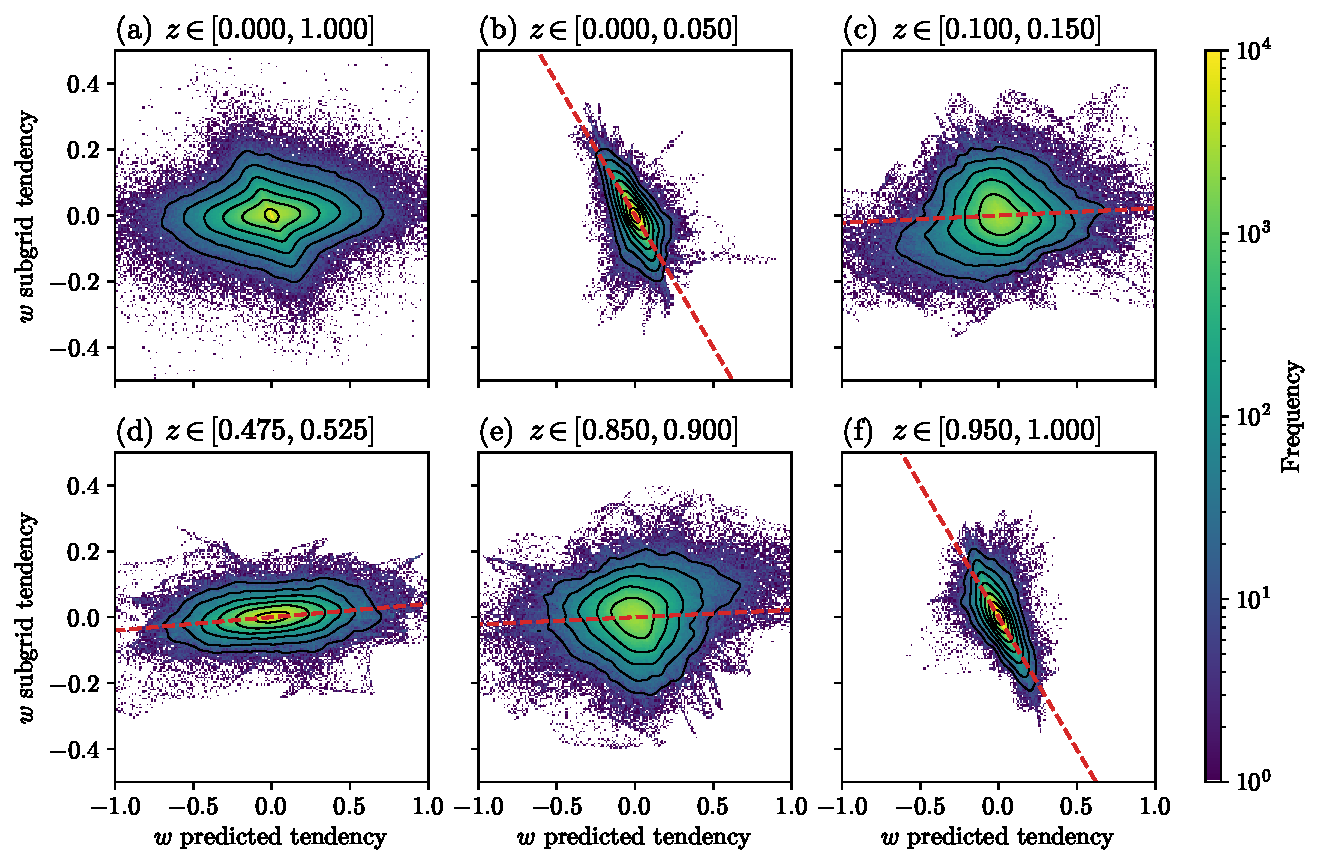
\includegraphics[width=0.95\linewidth]{figures/w_subgrid_vs_pred_tend.pdf}
    \caption{
        The equivalent of \cref{fig:theta_vs_w} for the $u$ subgrid
        tendency against the $u$ tendency predicted by the coarse model.
    }
    \label{fig:w_subgrid_vs_pred_tend}
\end{figure}


\section{Modelling of subgrid tendencies}
In \cref{sec:subgrid_analysis} I demonstrated several correlations that could
be exploited to construct a parametrisation scheme for modelling the subgrid
tendencies as functions of the coarse state variables. I choose to use the
relationship between subgrid tendencies and predicted tendencies, as it admits
a particularly simple parametrisation.

Observing that the subgrid tendencies (which I now denote by
$\mathcal{S}_\chi$, where $\chi = u, w, \theta$) are linearly correlated with
the predicted tendencies (denoted by $\mathcal{P}_\chi$) for any given $z$, I
propose a statistical model of the form
\begin{equation} \label{eqn:scheme}
    \mathcal{S}_\chi =  f_\chi(z)\,\mathcal{P}_\chi.
\end{equation}
The function $f_\chi(z)$ determines the slope of the linear relationship at
height $z$. \cref{eqn:scheme} is an attractive choice because it can be easily
coupled into the coarse model as a parametrisation scheme. To the right hand
side of the unparametrised coarse model equations $\partial \chi/\partial t =
\mathcal{P}_\chi,$ one simply adds the model for the subgrid tendencies,
meaning that the equations for the parametrised model are simply
\begin{equation} \label{eqn:res_tend_parametrised_model}
    \pdiff{\chi}{t} = \mathcal{P}_\chi + \mathcal{S}_\chi
        = [1 + f_\chi(z)] \mathcal{P}_\chi.
\end{equation}

It remains to determine $f_\chi(z)$. The conditional distributions in
\crefrange{fig:theta_subgrid_vs_pred_tend}{fig:w_subgrid_vs_pred_tend}
seem to be symmetric about $z=1/2$ (i.e., the histograms for $z \in [0, 0.05]$
and $z \in [0.1, 0.15]$ look very similar to those for $z \in [0.95, 1]$ and $z
\in [0.85, 0.9]$ respectively), so I assume that $f_\chi(z)$ is a polynomial
containing only even powers of $(z - 1/2)$. The statistical model
\cref{eqn:scheme} can then be expanded out as
\begin{equation} \label{eqn:scheme_poly}
    \mathcal{S}_\chi =
        \beta_0 \mathcal{P}_\chi + \beta_1 (z - 1/2)^2 \mathcal{P}_\chi
        + \beta_2 (z - 1/2)^4 \mathcal{P}_\chi + \cdots
        + \beta_N (z - 1/2)^{2N} \mathcal{P}_\chi,
\end{equation}
where $\beta_i$ are free parameters and $N$ determines the degree of the
polynomial. Because the model is linear in the $\beta_i$, it can be
efficiently fitted to the training data using ordinary least squares (OLS).

OLS fitting was performed using the \texttt{statsmodels} package in Python. A
choice of $N = 10$ for \cref{eqn:scheme_poly} was found to produce the best
fit. On top of each conditional histogram in
\crefrange{fig:theta_subgrid_vs_pred_tend}{fig:w_subgrid_vs_pred_tend}
I have plotted the line $\mathcal{S}_\chi =  f_\chi(z)\,\mathcal{P}_\chi$,
where $f_\chi$ is evaluated at the middle of the $z$ interval used for
conditioning. \cref{tab:r_squared} shows the coefficients of determination
$R^2$ for each variable. With $R^2 = 0.769$, the subgrid tendency of $\theta$
is captured fairly well. On the other hand, while
\cref{fig:u_subgrid_vs_pred_tend,fig:w_subgrid_vs_pred_tend} show that the fits
for $u$ and $w$ have the expected form (slope $f_\chi(z)$ close to -1 for $z$
near 0 and 1, and close to 0 elsewhere), their low coefficients of
determination indicate that the residuals are substantial and the use of
\cref{eqn:scheme_poly} is unlikely to add much value (especially for $w$).

\begin{table}[ht]
\centering
\begin{tabular}{l l}
    \toprule
    Variable & $R^2$ \\
    \midrule
    $\theta$ & 0.769 \\
    $u$ & 0.357 \\
    $w$ & 0.079 \\
    \bottomrule
\end{tabular}
\caption{
    Coefficients of detrmination $R^2$ for the OLS regression of each
    variable's subgrid tendency against its predicted tendency according to
    \cref{eqn:scheme_poly}.
}
\label{tab:r_squared}
\end{table}

Thus concludes the analysis and modelling of the subgrid tendencies;
\cref{eval-chap:evaluation} will take the next step of coupling the fitted
parametrisation scheme into the coarse model.


\ifSubfilesClassLoaded{%
    \emergencystretch=5em
    \printbibliography{}
}{}

\end{document}
